\chapter{Implementation\label{cha:chapter4}}
A proof of concept implementation of the concept introduced in \ref{cha:chapter3} is documented in this chapter. The code is available here: https://github.com/gurukeuck/Master-s-Thesis

\section{Sequence Diagrams}
\begin{figure}[ht]
	\centering
  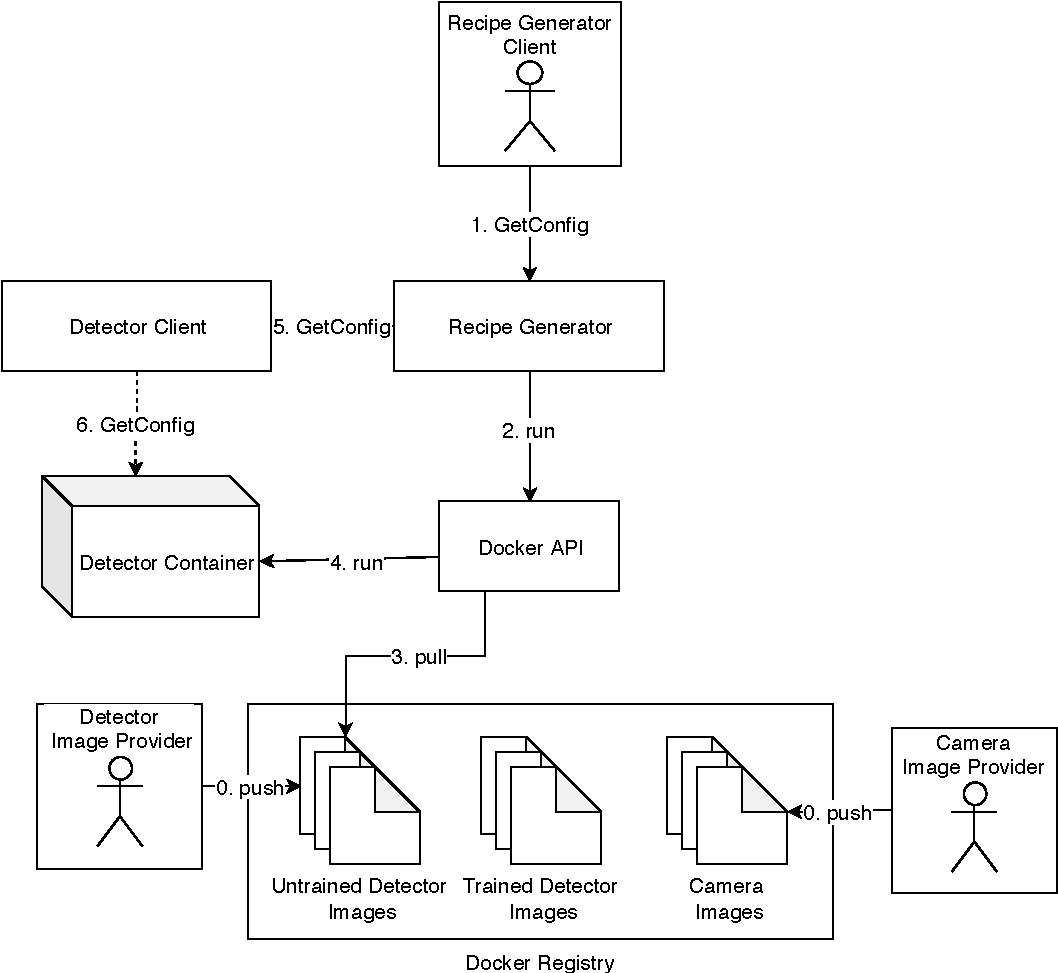
\includegraphics[width=\textwidth]{img/SequenceDiagram-GetConfig.pdf}
	\caption{Sequence Diagram - GetConfig}
	\label{fig:SequenceDiagram-GetConfig}
\end{figure}

\begin{figure}[ht]
	\centering
  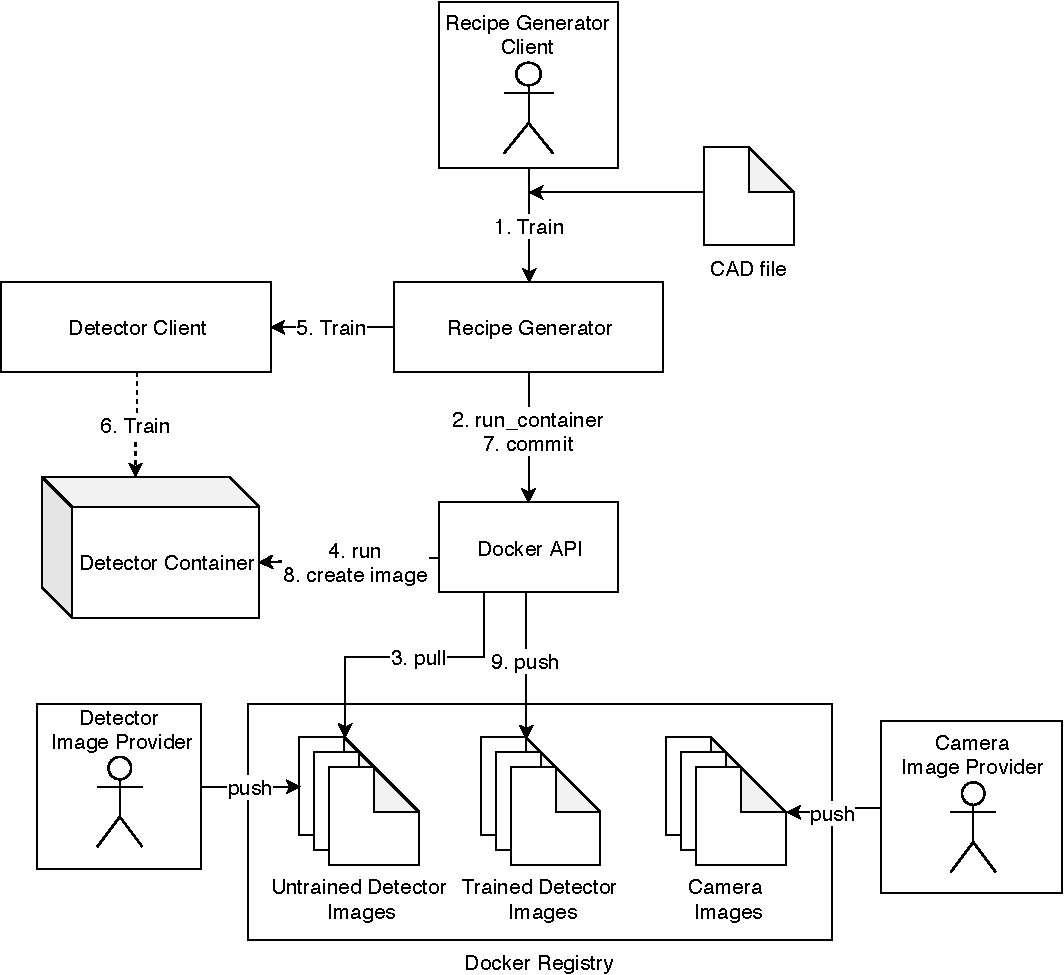
\includegraphics[width=\textwidth]{img/SequenceDiagram-Train.pdf}
	\caption{Sequence Diagram - Train}
	\label{fig:SequenceDiagram-Train}
\end{figure}

\begin{figure}[ht]
	\centering
  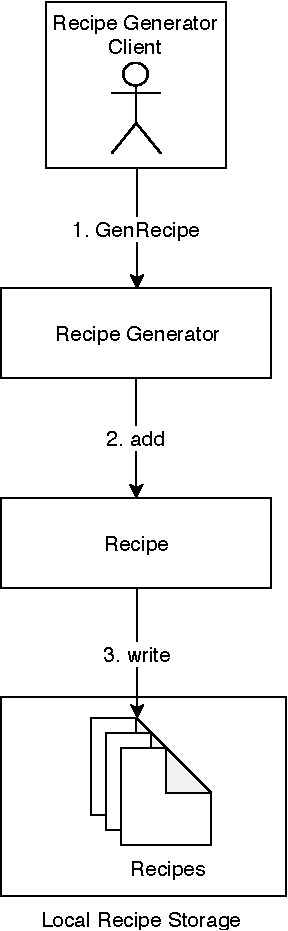
\includegraphics[height=0.6\textheight]{img/SequenceDiagram-GenRecipe.pdf}
	\caption{Sequence Diagram - GenRecipe}
	\label{fig:SequenceDiagram-GenRecipe}
\end{figure}

\begin{figure}[ht]
	\centering
  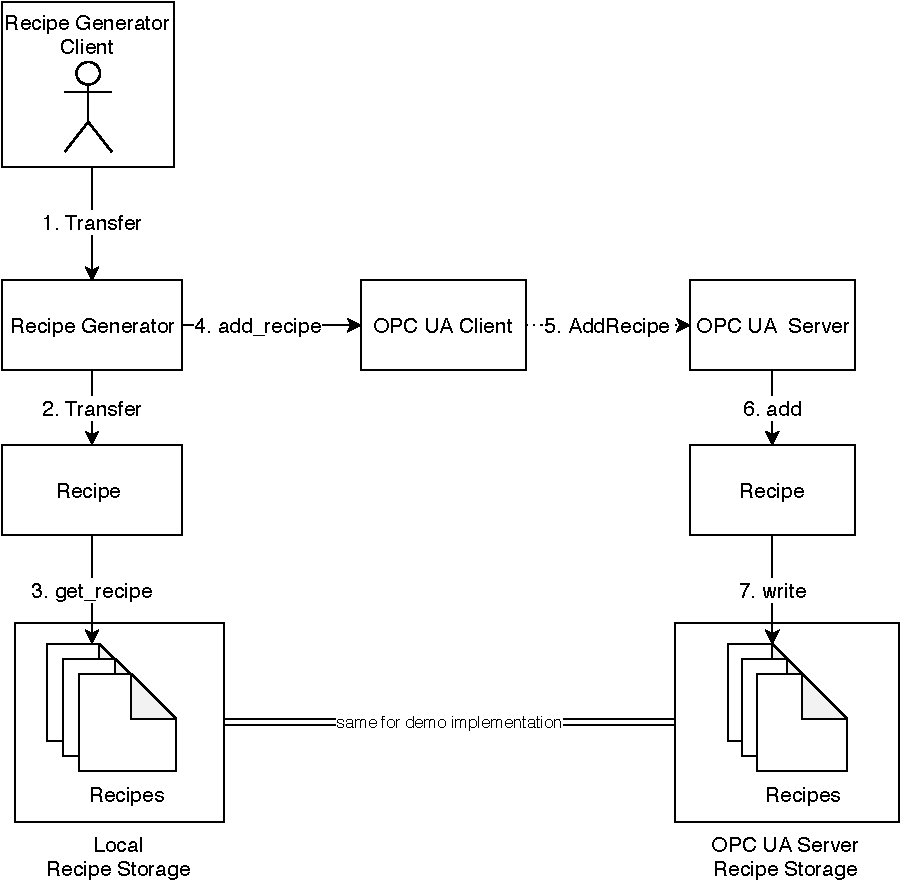
\includegraphics[width=\textwidth]{img/SequenceDiagram-Transfer.pdf}
	\caption{Sequence Diagram - Transfer}
	\label{fig:SequenceDiagram-Transfer}
\end{figure}

\begin{figure}[ht]
	\centering
  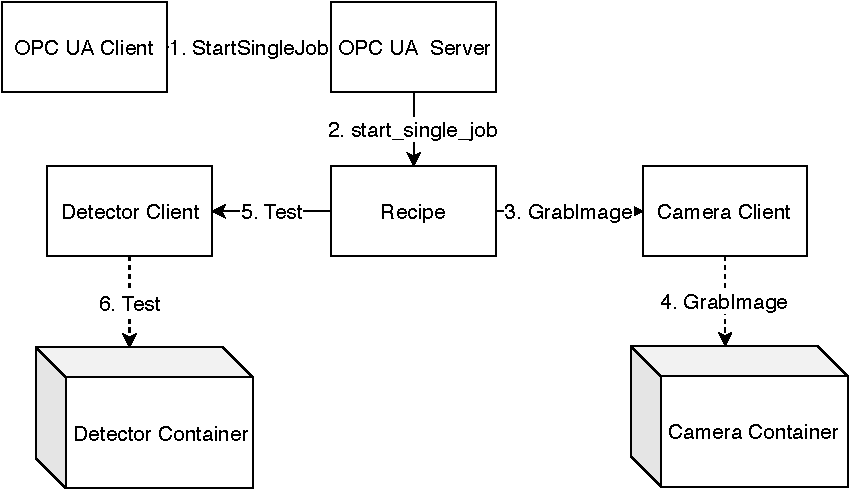
\includegraphics[width=\textwidth]{img/SequenceDiagram-Test.pdf}
	\caption{Sequence Diagram - Test}
	\label{fig:SequenceDiagram-Test}
\end{figure}

\section{Class diagram}
\begin{figure}[ht]
	\centering
  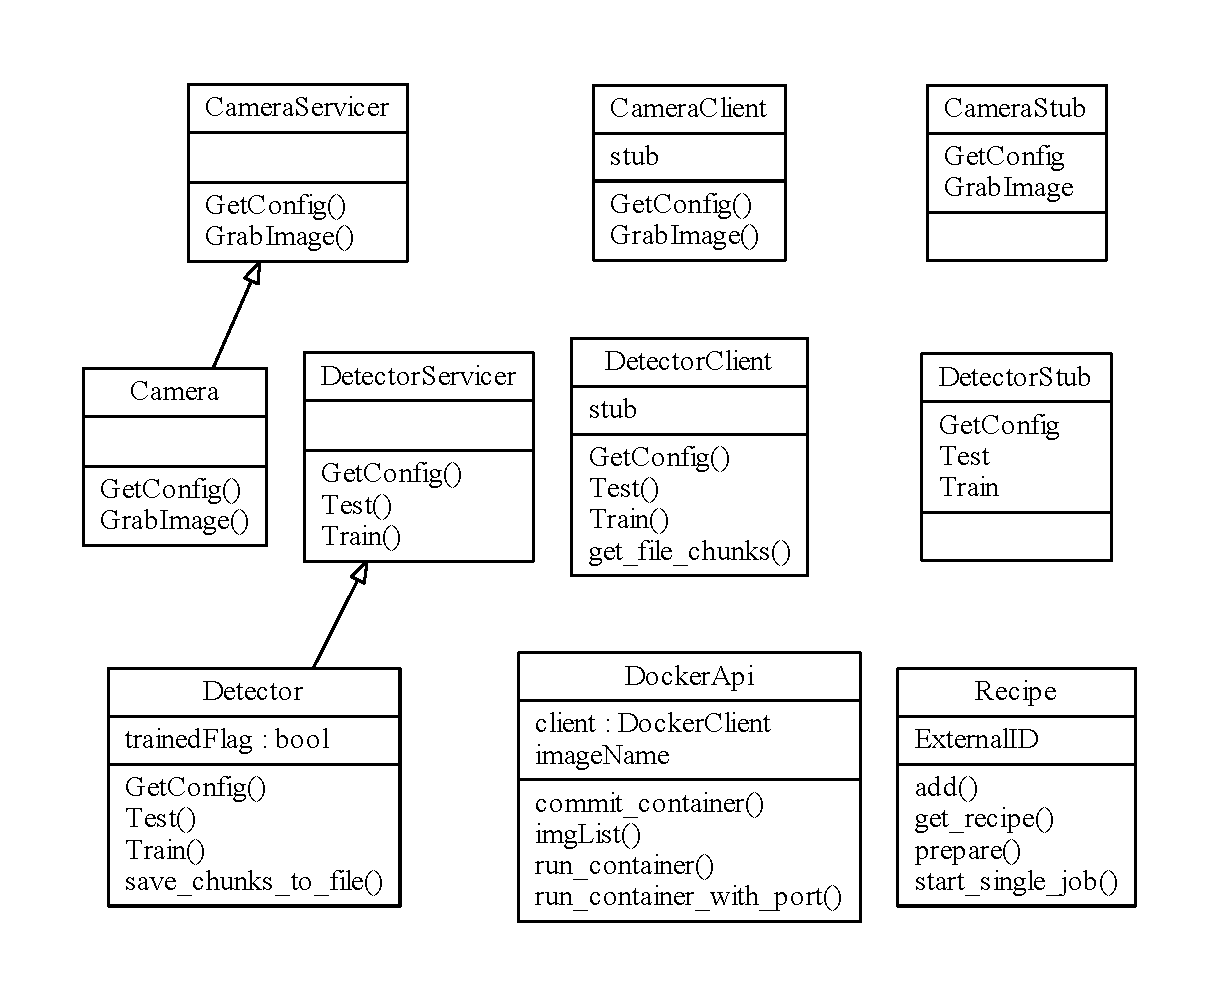
\includegraphics[width=\textwidth]{img/classes.pdf}
	\caption{Class diagram}
	\label{fig:Classes}
\end{figure}

\section{Package diagram}
\begin{figure}[ht]
	\centering
  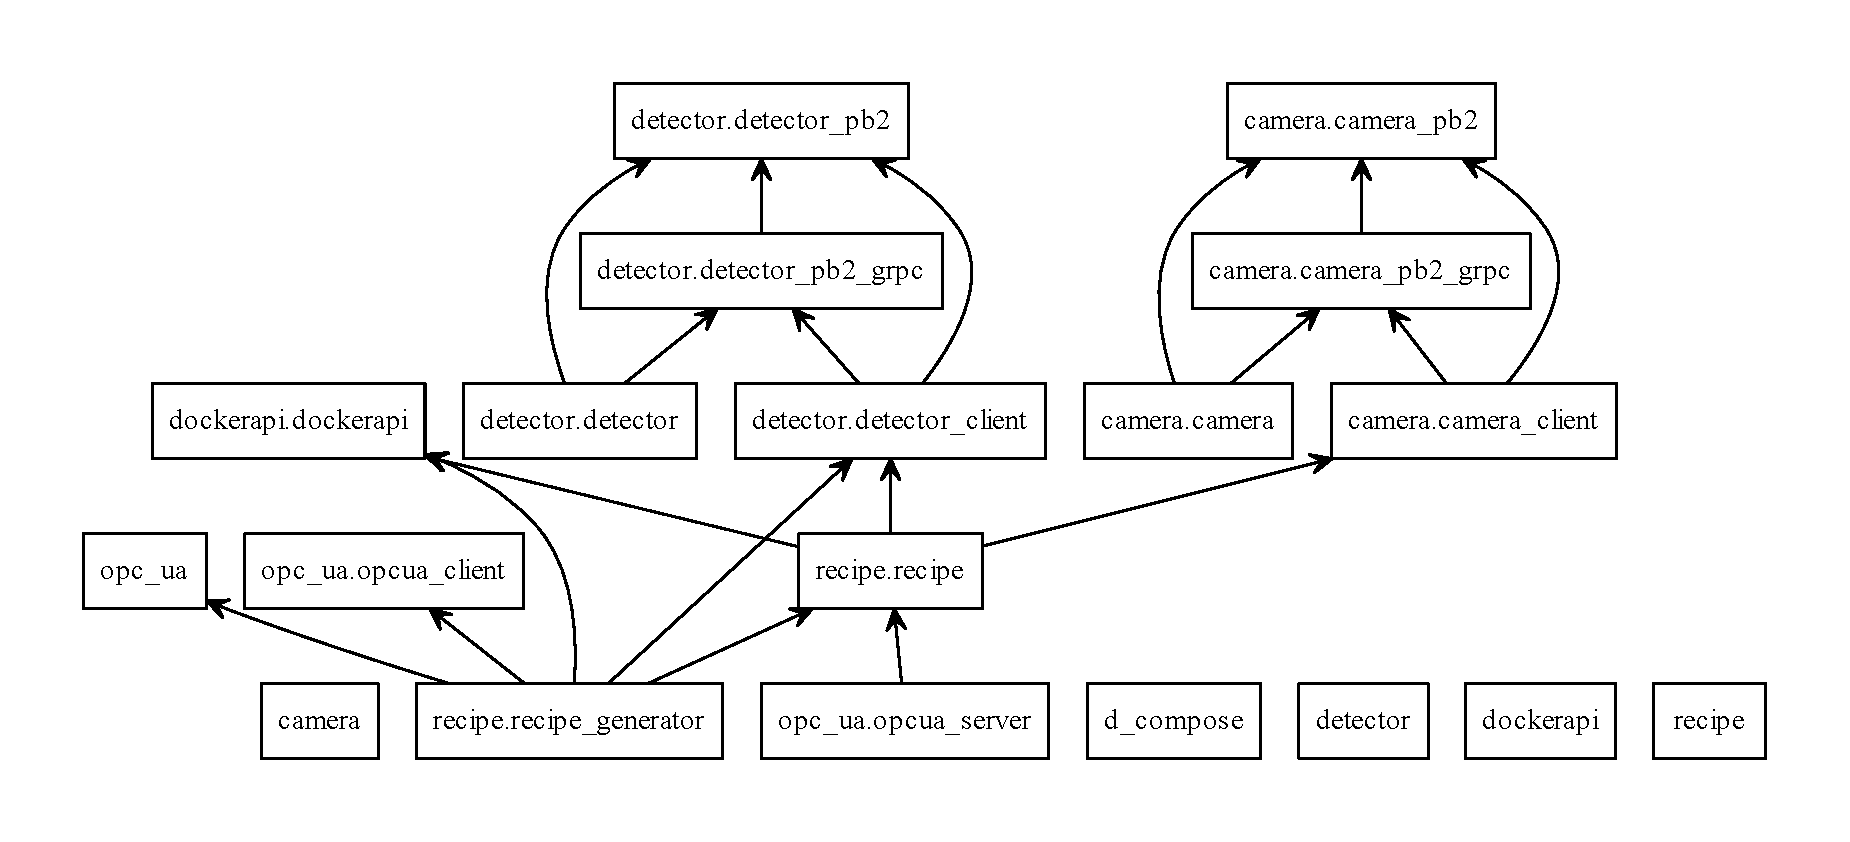
\includegraphics[width=\textwidth]{img/packages.pdf}
	\caption{Package diagram}
	\label{fig:Packages}
\end{figure}

\section{Virtualization Technology: Docker}
Realizing a SOA calls for means of decoupling the components and efficient tooling. Docker is the technology which was used here due to following reasons:
\subsection{Dependencies of components are handled smoothly} 
Every docker image can pull the packages and system variables it needs as specified in the dockerfile. E.g. one detector may depend on openCV 2.7.1 while another detector depends on 1.8. Both docker images that are built using their respective dockerfile are independent of each other. If no virtualization technology would be used here, a dependency handling for the whole recipe management would be necessary. In the case of two openCV versions just a slight modification of the framework may be necessary. A more drastic example would be detectors that rely on different .NET frameworks which might not be able to coexist on a system.
\subsection{Platform Independency}
 A platform in this context means operating system, e.g. Windows or Linux. The independency is twofold. Firstly, the docker engine runs on Linux (CentOS, Debian, Fedora, Oracle Linux, RHEL, SUSE and Ubuntu) and Windows Server. In an industrial context, both platforms are present and should be supported for maximum flexibility.
\subsection{Orchestration}
 Containers can be scaled if more resources are needed, an extensive monitoring is possible and the network over which the containers communicate can be configured. 
\subsection{Docker Hub}
 Docker offers (semi)-public or private repositories. They can be used by detector or camera providers to push their docker images and for the recipe management to pull them. As base image there are preconfigured environments available. For this implementation a fully functioning python environment was used as base docker image. To prevent know-how leaking of detection methods the accessibility to the images on the hub can be restricted. In this implementation a local repository was used with full accessibility to the docker images.
 \subsection{Calculations on Graphical Processing Unit}
 Some detectors need excessive calculation power. If applicable, the graphical processing unit of the bare metal server the docker engine is running on can be added. It should be kept in mind that with this technique the detector docker image is dependent not only on the docker engine but also the bare metal hardware. Thus, this option should be used with caution and only if needed.
\subsection{Reason against Docker}
The reason against using Docker is making all involved parties introduced in \ref{sec:involvedparties} use docker. Camera and detector docker image providers need to add a dockerfile for building the image and pushing it to the repository. On the recipe management side a docker engine compatible infrastructure has to be provided. 

\section{Inter-Service Communication: gRPC}
In the current implementation this is static. Detectors listen on port 8000, cameras on port 8011. 

\section{Programming Language: Python}
For implenting a proof of the concept created in \ref{cha:chapter3}, a programming language meeting multiple requirements is mandatory. 

\subsection{Support for Docker}


\subsection{Support for gRPC}

\subsection{Support for OPC UA}

\section{Object Detection Methods used}
dummy!

\section{Differences to OPC UA Vision Specification}